\subsection{Modelos basados en redes neuronales}

A partir de 1986\cite{Rumelhart_1987}, los modelos conexionistas o redes neuronales han sido utilizados como herramientas de predicción y clasificación. Un modelo basado en redes neuronales es un sistema informático que mediante el uso de pesado auto-modificable.

\paragraph{Perceptrón}

El perceptrón fue propuesto por Frank Rosenblatt\cite{Rosenblatt_1958}. El modelo más básico de una neurona es un perceptrón. El perceptrón usa una matriz para representar las redes neuronales, esta matriz es llamada matriz de pesos o solamente pesos. Las componentes de un modelo perceptrón son la capa de entrada, la capa oculta, una función de activación y la salida. En la capa oculta es donde se calcula la mutiplicación con la matriz de pesos. En la tabla \ref{table:activation_functions} se encuentran las funciones más usadas como funciones de activación.

\begin{table}[H]
	\centering
	\begin{tabular}{ll} \hline
		\textbf{Función} & \textbf{Definición}         \\ \hline
		Lineal           & $f(x)=x$                    \\[0.1cm]
		Sigmoide         & $f(x)=\frac{1}{1+e^{-x}}$   \\[0.1cm]
		ReLU             & $f(x)=\begin{cases}
				                         0 & \text{si x}<0     \\
				                         x & \text{si x}\leq 0 \\
			                         \end{cases}$ \\ [0.1cm]
		Tanh             & $f(x)=tanh(x)$              \\ [0.1cm] \hline
	\end{tabular}
	\caption{Funciones de activación comúnmente usadas.}
	\label{table:activation_functions}
\end{table}

El perceptrón multicapa tiene una estructura similar a la de un modelo perceptrón. En este caso se incluyen capas ocultas donde todas se encuentran conectadas, a esto se le denomina como una capa densa. En cada iteración existe una actualización con propagación hacia atras en las capas densas para entrenar el modelo. En nuestro caso se implemento un perceptrón multicapa con tres capas de 256, 128 y 3 capas densas con la función de activación sigmoide. En la figura \ref{fig:perceptron} se representa de manera visual el modelo perceptrón.

\begin{figure}[H]
	\centering
	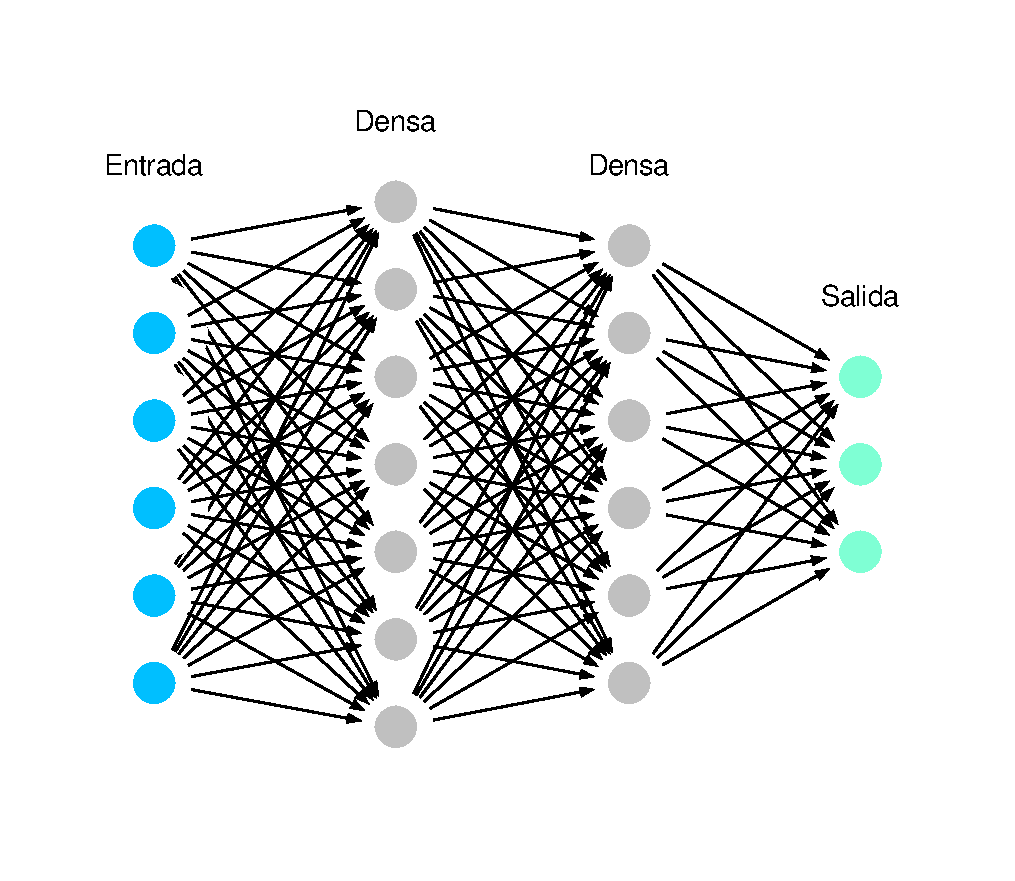
\includegraphics[width=10cm]{Graphics/perceptron.pdf}
	\caption{Representación del modelo perceptrón multicapa\cite{dotnet}.}
	\label{fig:perceptron}
\end{figure}

\paragraph{Red Recurrente}

Las redes neuronales recurrentes son una clase de redes neuronales que permiten conocer la salida anterior y utilizarla conociendo sus pesos. Para cada tiempo t, la función de activación ($a_t$) y la salida ($y_t$) son expr

\paragraph{Red Convolucional}
\paragraph{Long short-term memory}
\paragraph{Bidireccional Long-short-term memory}
\paragraph{Red convolucional con atención}
\paragraph{Esquema de votación}
